\chapter{Analiza istniejących platform do automatyki budynkowej}
Na rynku już istnieją platformy i do tego darmowe więc można uznać że zapotrzebowanie na taką platformę nie istnieje. W związku z tym można uznać że potencjał biznesowy jest również niewielki. Systemy takie jak Home-assistant Rys.  \ref{fig:homeAssistant}, Domoticz Rys. \ref{fig:domoticz} lub Node-red są darmowe z otwartym kodem źródłowym. Warto jednak tutaj wspomnieć że próbują na swój sposób zarabiać i taki na przykład Home Assistant proponuje usługę chmury gdzie użytkownik integruje swoje systemy przez panel administratora i są mu udostępniane pomocne dodatki takie jak usługa Google Assistant.  
Te produkty róznie podchodzą do tematu, ale skupiają się na tej samej tematyce. Analizując ich działanie można znaleźć takie problemy jak:
\begin{itemize}
    \item ograniczona ingerencja w logikę systemu
    \item trudność z integracją urządzeń których producent platformy nie przewidział
    \item przestarzałe technologie
    \item toporność działania
\end{itemize}
Przez tą różnorodność użytkownicy są rozdzieleni między tymi platformami i każdy wybiera coś dla siebie.
Oprócz tego wiele komercyjnych sterowników przekaźnikowych udostępnia aplikacje mobilne do integracji produktów dla tej samej marki co jest jednocześnie głównym problemem. Takie rozwiązania proponuje Shelly, Sonoff, Xiaomi smart-home. Platformy te są również odpowiedzią dla bardzo drogich komercyjnych jednostek przeznaczonych  głównie dla domów inteligentnych działających w strukturze KNX. 
\par Tworząc platformę pewne elementy zostały zaczerpnięte z istniejących produktów, natomiast niektóre elementy mogą zostać zrobione lepiej. Do tematu wrócę jeszcze w rozdziale 4.

\begin{figure}[h]
  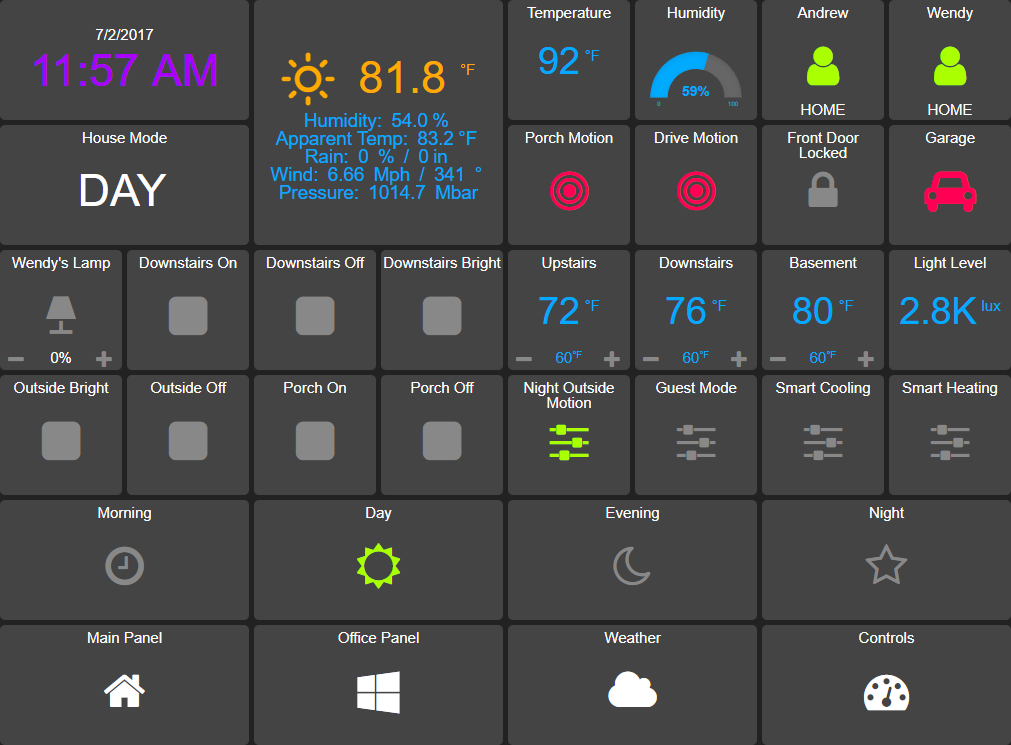
\includegraphics[width=\linewidth]{homeAssistant.png}
  \caption{HomeAssistant}
  \label{fig:homeAssistant}
\end{figure}

\begin{figure}[h]
  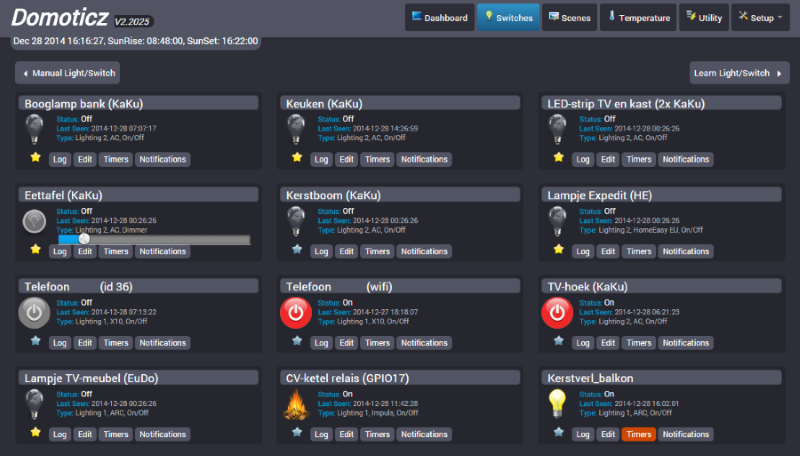
\includegraphics[width=\linewidth]{domoticz.png}
  \caption{Domoticz}
  \label{fig:domoticz}
\end{figure}